\documentclass[addpoints,12pt]{exam}
\usepackage[utf8]{inputenc}
\usepackage[spanish,es-noshorthands]{babel}
\usepackage{amsmath,amssymb}
\usepackage{graphicx}
\usepackage{array}
\usepackage{xcolor}
\usepackage{tikz}
\usetikzlibrary{calc,arrows.meta,decorations.markings}
\usepackage[most]{tcolorbox}
\usepackage[legalpaper,margin=2cm,top=1.8cm]{geometry}

\graphicspath{{./}}
\definecolor{ubbblue}{RGB}{0,51,102}
\definecolor{cargazul}{RGB}{40,40,210}
\definecolor{cargarojo}{RGB}{210,40,40}

\qformat{}
\newcommand{\qpts}[1]{{\setlength{\fboxsep}{2.5pt}\fbox{#1}}\hspace{0.6em}\ignorespaces}
\newcommand{\qhead}[1]{\thequestion.\hspace{0.5em}\qpts{#1}}
\newcommand{\pts}[1]{\textcolor{red}{\textbf{(#1 pts)}}}

\pagestyle{headandfoot}
\runningheadrule
\firstpageheader{}{}{}
\runningheader{\small F\'isica II - Electromagnetismo}%
              {\small\textbf{Certamen 2}}%
              {\small 25 de Septiembre, 2026}
\firstpagefooter{}{\thepage}{}
\runningfooter{}{Page \thepage\ of \numpages}{}

\begin{document}

%========================================================
% PORTADA
%========================================================
\begin{center}
    
\includegraphics[height=1.9cm]{logo ubb.png}\hspace{1cm}%
    
\includegraphics[height=1.5cm]{logo dfis.png}\\[0.5cm]
    {\Large F\'isica II - Electromagnetismo}\\[0.15cm]
    {\LARGE\textbf{Certamen 2}}\\[0.9cm]
    25 de Septiembre, 2026
\end{center}

\vspace{0.7cm}

\noindent\textbf{Nombre Completo}: \hrulefill\\[0.7cm]
\noindent\textbf{Rut}: \makebox[6.5cm]{\hrulefill}\hspace{0.3cm}\textbf{Carrera}: \hrulefill

\vspace{0.4cm}
\noindent\rule{\textwidth}{1pt}
\vspace{0.2cm}

\noindent\textbf{Algunas consideraciones para esta evaluaci\'on:}
\begin{itemize}\setlength\itemsep{2pt}
    \item El certamen 2 contiene \numpages\ p\'aginas (incluida la portada) y \numquestions\ preguntas,
          con un total de \numpoints\ puntos.
    \item Cada pregunta debe ser respondida por s\'olo una respuesta. En caso de presentar m\'as de
          una, se anulan las respuestas.
    \item \textbf{No est\'a permitido el uso de celulares o tablet en el desarrollo de esta
          evaluaci\'on. De ser sorprendido utilizando estos art\'iculos su evaluaci\'on ser\'a
          calificada con nota 1.0.}
    \item Buena suerte!
\end{itemize}

\noindent Seleccione con una \textbf{X} el nombre del profesor de su secci\'on:

\vspace{0.15cm}
\noindent
\begin{minipage}{0.49\textwidth}
\begin{tabular}{|l|p{1.1cm}|}
\hline
Prof.\ Luis Soto & \\ \hline
Prof.\ Evelyn Riveros & \\ \hline
Prof.\ Bayron Cerda & \\ \hline
Prof.\ Luis Liempi & \\ \hline
\end{tabular}
\end{minipage}%
\begin{minipage}{0.49\textwidth}
\begin{tabular}{|l|p{1.1cm}|}
\hline
Prof.\ Natalia Molina & \\ \hline
Prof.\ Ricardo Espinoza & \\ \hline
Prof.\ Crist\'obal Gatica & \\ \hline
~ & \\ \hline
\end{tabular}
\end{minipage}

\vspace{0.9cm}
\begin{center}
{\large\textbf{Puntaje}}\\[0.2cm]
\gradetable[v][questions]
\end{center}

\newpage

%========================================================
% PREGUNTAS
%========================================================
\begin{questions}

%--------------------------------------------------------
% PREGUNTA 1  (P1 Gauss coaxial - misma en ambas formas)
%--------------------------------------------------------
\question[22]
\begin{minipage}[t]{0.56\textwidth}
\vspace{0pt}
\qhead{22}Considere dos cilindros coaxiales muy largos, ambos de longitud $H$.
\begin{itemize}\setlength\itemsep{1pt}
    \item El \textbf{cilindro interior} es un conductor macizo de radio $R$, con carga total $+Q$.
    \item El \textbf{cilindro exterior} es un aislante que ocupa la regi\'on entre $2R$ y $3R$, con carga
          total $-2Q$ distribuida uniformemente en su volumen.
    \item Entre $R$ y $2R$ existe espacio vac\'io.
\end{itemize}
Con una superficie gaussiana cil\'indrica coaxial de radio $r$ y longitud $L$ ($L<H$; se desprecian los
extremos), aplique la Ley de Gauss para determinar el campo eléctrico en las regiones:
\end{minipage}\hfill
\begin{minipage}[t]{0.46\textwidth}
\vspace{0pt}
\centering
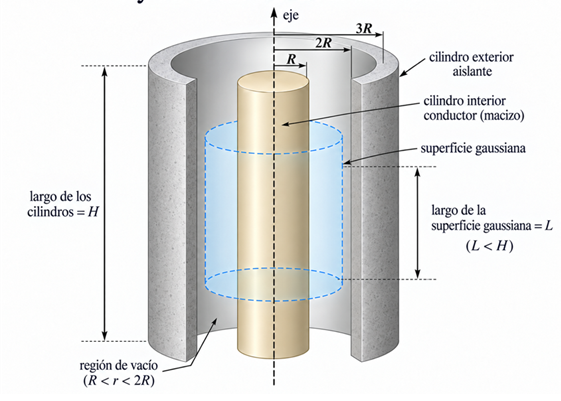
\includegraphics[width=\textwidth]{figura gauss forma b.png}\\[2pt]
{\footnotesize Fig.\ 1.}
\end{minipage}

\medskip
\noindent\textbf{(a)} Regi\'on $r<R$. \pts{4}

\vspace{5.2cm}
\noindent\textbf{(b)} Regi\'on $R<r<2R$. \pts{6}

\vspace{5cm}
\noindent\textbf{(c)} Regi\'on $2R<r<3R$. \pts{8}

\vspace{4cm}
\noindent\textbf{(d)} Regi\'on $r>3R$. \pts{4}

\newpage

%--------------------------------------------------------
% PREGUNTA 2  (P2 version 2 = main2)
%--------------------------------------------------------
\question[17]
\begin{minipage}[t]{0.56\textwidth}
\vspace{0pt}
\qhead{17}Se dispone de un sistema formado por 3 cargas puntuales: $q_1=-12$ [nC], $q_2=25$ [nC] y
$q_3=-6$ [nC] ubicadas en los puntos $P_1(0,6,6)$, $P_2(4,0,3)$ y $P_3(4,4,4)$ respectivamente, como muestra la Figura. Si las
posiciones est\'an expresadas en cent\'imetros,
\end{minipage}\hfill
\begin{minipage}[t]{0.40\textwidth}
\vspace{0pt}
\centering
\begin{tikzpicture}[scale=0.72]
    \draw[step=1cm,very thin, gray!40] (-4,-3) grid (4,4);
    \draw[black, line width =1.1,->, >=latex] (0,0) -- (0,4) node [black, right] {$Y$};
    \draw[black, line width =1.1,->, >=latex] (0,0) -- (4,0) node [black, above] {$X$};
    \draw[black,line width=1.1, ->, >=latex] (0,0) -- (-3,-2.2) node [black, above] at (-3.2,-2.3) {$Z$};
    \node[black, right] at (-2.8,-1.2) {$P$};
    \fill (-2,-1.5) circle (0.16);
    \node[black,left] at (0,3) {$6$};
    \fill (-2,1.8) circle (0.16);
    \draw[black, dashed] (0,3) -- (-2,1.8) node[black] at (-2.5,1.8) {$q_1$};
    \draw[black, dashed] (-2,1.8) -- (-2,-1.5) node[black] at (-2,-2.2) {$6$};
    \draw[black, dashed] (2,0) -- (1,-1.2) node[black, below] at (2,0) {$4$};
    \draw[black, dashed] (1,-1) -- (-1.2,-1) node[black] at (-1.5,-0.6) {$3$};
    \fill (1,-1) circle (0.16);
    \node[black,below] at (1.2,-1.1) {$q_2$};
    \draw[black, dashed] (0,2) -- (2,2) node[black, left] at (0,2) {$4$};
    \draw[black, dashed] (2,0) -- (2,2);
    \draw[black, dashed] (0.7,-1.2) -- (-1.6,-1.2) node[black] at (-1.5,-1.4) {$4$};
    \draw[black, dashed] (0.8,0.9) -- (2,2);
    \draw[black, dashed] (0.8,-1.2) -- (0.8,0.9);
    \draw[black, dashed] (-1.7,-1.1) -- (-1.7,0.9);
    \draw[black, dashed] (-1.7,0.9) -- (0.8,0.9);
    \draw[black, dashed] (-1.7,0.9) -- (0,2);
    \node[black,below] at (1.3,1) {$q_3$};
    \fill (0.8,0.9) circle (0.16);
\end{tikzpicture}\\[2pt]
{\footnotesize Fig.\ 2 (posiciones en cm).}
\end{minipage}

\medskip
\noindent\textbf{(a)} Calcule el potencial el\'ectrico en el punto $P(0,0,6)$. \pts{7}

\vspace{6cm}
\noindent\textbf{(b)} Calcule la energ\'ia contenida en el sistema. \pts{7}

\vspace{6.5cm}
\noindent\textbf{(c)} Calcule el trabajo necesario para traer una carga $q_4=14$ [nC] al punto $P$. \pts{3}

\newpage

%--------------------------------------------------------
% PREGUNTA 3  (P3 version 2 = uniforme v2)
%--------------------------------------------------------
\question[20]
\begin{minipage}[t]{0.56\textwidth}
\vspace{0pt}
\qhead{20}En el plano $xy$ se tiene un arco de circunferencia de radio $R$, centrado en el origen $O$ y
con densidad lineal de carga uniforme $\lambda_1$. A partir del punto del arco ubicado sobre el eje $x$
negativo se extiende una barra recta de longitud $2R$, con densidad lineal de carga uniforme $\lambda_0$.
\end{minipage}\hfill
\begin{minipage}[t]{0.40\textwidth}
\vspace{0pt}
\centering
\begin{tikzpicture}[scale=0.82]
    \def\R{1.45}
    \draw[->,thick] (-5.0,0) -- (1.35,0) node[right] {$x$};
    \draw[->,thick] (0,-2.0) -- (0,2.05) node[above] {$y$};
    \fill (0,0) circle (1.2pt);
    \node[below right] at (0,0) {$O$};
    \draw[line width=1.6pt] (135:\R) arc[start angle=135, end angle=225, radius=\R];
    \draw[densely dashed] (0,0) -- (135:\R);
    \draw[densely dashed] (0,0) -- (225:\R);
    \node[font=\small] at (-0.62,0.27) {$45^\circ$};
    \node[font=\small] at (-0.62,-0.27) {$45^\circ$};
    \node[left,font=\small] at (-0.6,1.25) {$\lambda_1$};
    \node[right,font=\small] at (-0.78,-0.95) {$R$};
    \draw[line width=2.5pt] ({-3*\R},0) -- (-\R,0);
    \draw (-\R,0.11) -- (-\R,-0.11);
    \draw ({-3*\R},0.11) -- ({-3*\R},-0.11);
    \node[above,font=\small] at ({-2*\R},0.20) {$\lambda_0$};
    \draw[<->] ({-3*\R},-0.48) -- (-\R,-0.48);
    \node[fill=white, inner sep=1pt,font=\small] at ({-2*\R},-0.48) {$2R$};
\end{tikzpicture}\\[2pt]
{\footnotesize Fig.\ 3.}
\end{minipage}

\medskip
\noindent\textbf{(a)} Determine el potencial el\'ectrico total en el origen $O$ debido a ambas distribuciones, en función de $\lambda_0$ y $\lambda_1$. \pts{12}

\vspace{7.5cm}
\noindent\textbf{(b)} Determine el valor de $\lambda_0$, en funci\'on de $\lambda_1$, para que el potencial total en el origen $O$ sea cero. \pts{3}

\vspace{3cm}
\noindent\textbf{(c)} Con el $\lambda_0$ anterior, determine la carga el\'ectrica total de ambas distribuciones en funci\'on de $\lambda_1$. \pts{5}

\end{questions}

\newpage

%========================================================
% FORMULARIO
%========================================================
\newtcolorbox{formbox}[1]{colback=gray!3, colframe=gray!55, coltitle=white,
    colbacktitle=gray!45, fonttitle=\bfseries, boxrule=0.5pt, arc=2pt,
    left=6pt,right=6pt,top=2pt,bottom=2pt, before skip=4pt, after skip=4pt,
    title={#1}}
\setlength{\jot}{2pt}

\begin{center}{\large\textbf{Formulario}}\end{center}
\vspace{-0.1cm}
{\centering\footnotesize $k=\dfrac{1}{4\pi\varepsilon_0}=9\times10^{9}\ \mathrm{N\,m^2/C^2}$,\quad
$\varepsilon_0=8{,}85\times10^{-12}\ \mathrm{C^2/(N\,m^2)}$\par}

\begin{formbox}{Ley de Gauss}
\[
    \oint \vec E\cdot d\vec S=\frac{Q_{enc}}{\varepsilon_0}
\]
\end{formbox}

\begin{formbox}{Potencial el\'ectrico}
\[
    V=k\int\frac{dq}{r}\ ;\qquad V=k\,\frac{q}{r}\ ;\qquad V=k\sum_i\frac{q_i}{r_i}
\]
\end{formbox}

\begin{formbox}{Energ\'ia de un sistema de cargas y trabajo}
\[
    U=k\sum_{i<j}\frac{q_i q_j}{r_{ij}}\ ;\qquad W_{a\to b}=q\,(V_a-V_b)\ ;\qquad W_{\infty\to P}=q\,V_P
\]
\end{formbox}

\begin{formbox}{Densidades de carga}
\[
    \lambda=\frac{dq}{d\ell}\ ;\qquad \sigma=\frac{dq}{dA}\ ;\qquad \rho=\frac{dq}{dV}
\]
\end{formbox}

\begin{formbox}{Cilindro de largo $L$ y radio $R$}
\[
    V_{\text{cil}}=\pi R^{2}\,L\ ;\qquad A_{\text{manto}}=2\pi R\,L
\]
\end{formbox}

\begin{formbox}{Integrales t\'ipicas}
\noindent
\begin{minipage}{0.5\textwidth}
\begin{itemize}\setlength\itemsep{1pt}
    \item $\displaystyle\int \frac{dx}{x}=\ln|x|+C$
    \item $\displaystyle\int x\,dx=\frac{x^2}{2}+C$
    \item $\displaystyle\int d\theta=\theta+C$
\end{itemize}
\end{minipage}%
\begin{minipage}{0.48\textwidth}
\begin{itemize}\setlength\itemsep{1pt}
    \item $\displaystyle\int \cos\theta\,d\theta=\sin\theta+C$
    \item $\displaystyle\int \sin\theta\,d\theta=-\cos\theta+C$
    \item $\sin\tfrac{\pi}{4}=\cos\tfrac{\pi}{4}=\tfrac{\sqrt2}{2}$
\end{itemize}
\end{minipage}
\end{formbox}

\begin{formbox}{Prefijos}
$c=10^{-2}$, \quad $m=10^{-3}$, \quad $\mu=10^{-6}$, \quad $n=10^{-9}$, \quad $p=10^{-12}$.
\end{formbox}

\end{document}
